\chapter{Introduction}
\label{introduction}

Folding clothes is a common and necessary, but tedious, task for humans. Additionally, due to the increasing aging of the world population, a growing need exists for 
\juansays{automated solutions}
to be able to help us with laundry. Current automated solutions, shown in Figure \ref{fig:current_solutions}, are bulky, expensive, and require a large dedicated space, as they are intented to be used in an industrial environment. Also, due to the complexity of the garment manipulation task,  these solutions are designed to be integrated into an \juansays{assembly line}, with several machines chained to perform the whole process. Therefore, they are not suitable for domestic use. The proposed alternative is to use a robot to perform these \comment{laundry manipulation} tasks. A humanoid robot, designed to work in human environments, and to have human-like locomotion and manipulation capabilities seems to be a sensible choice.

%\begin{figure}[htbp]
%    \centering
%    
\includegraphics[width=0.8\textwidth]{figures/placeholder2.png}
%    \caption{\comment{Current clothes folding solutions}}
%    \label{fig:current_solutions}
%\end{figure}

\begin{figure}[htbp]
		\centering
        \begin{subfigure}[l]{0.42\textwidth}
            \centering
    		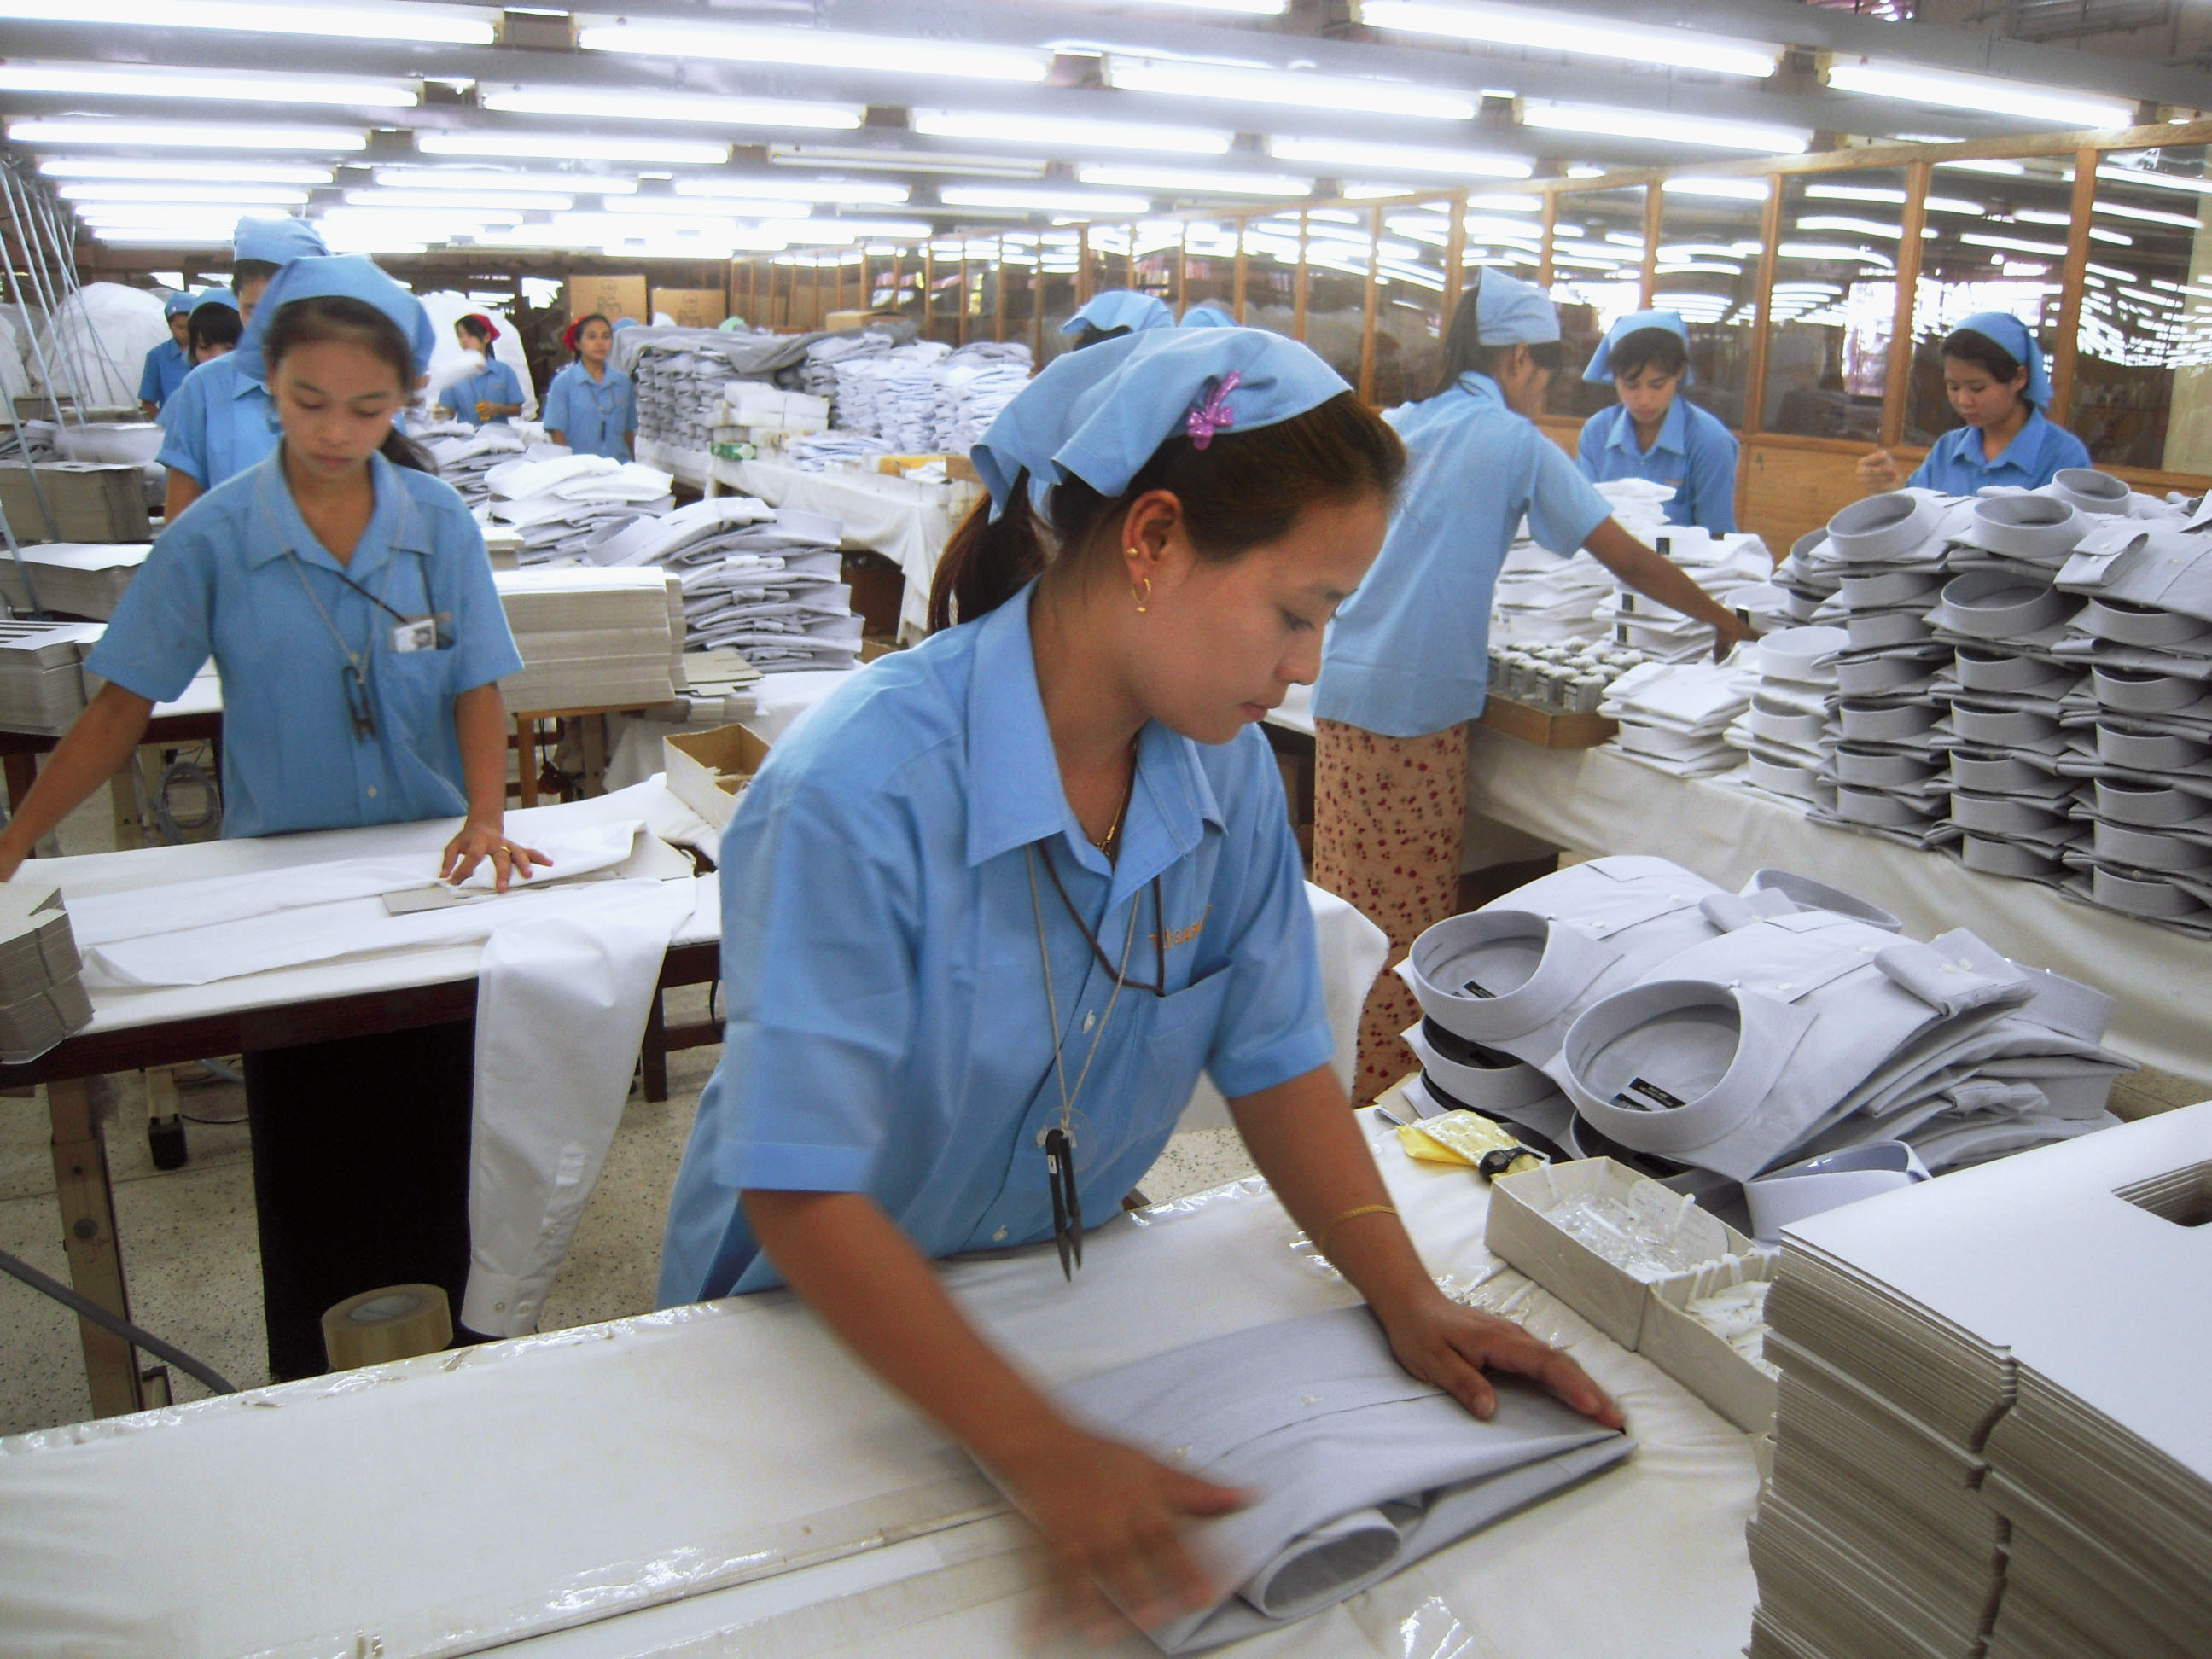
\includegraphics[width=\textwidth]
    		{figures/Intro_japan_folding.jpg}
			\caption{Human-based folding} %http://www.japantimes.co.jp/news/2012/12/19/reference/firms-move-some-eggs-out-of-china-basket/
        \end{subfigure}
        ~
        \begin{subfigure}[r]{0.56\textwidth}
	        \centering
    		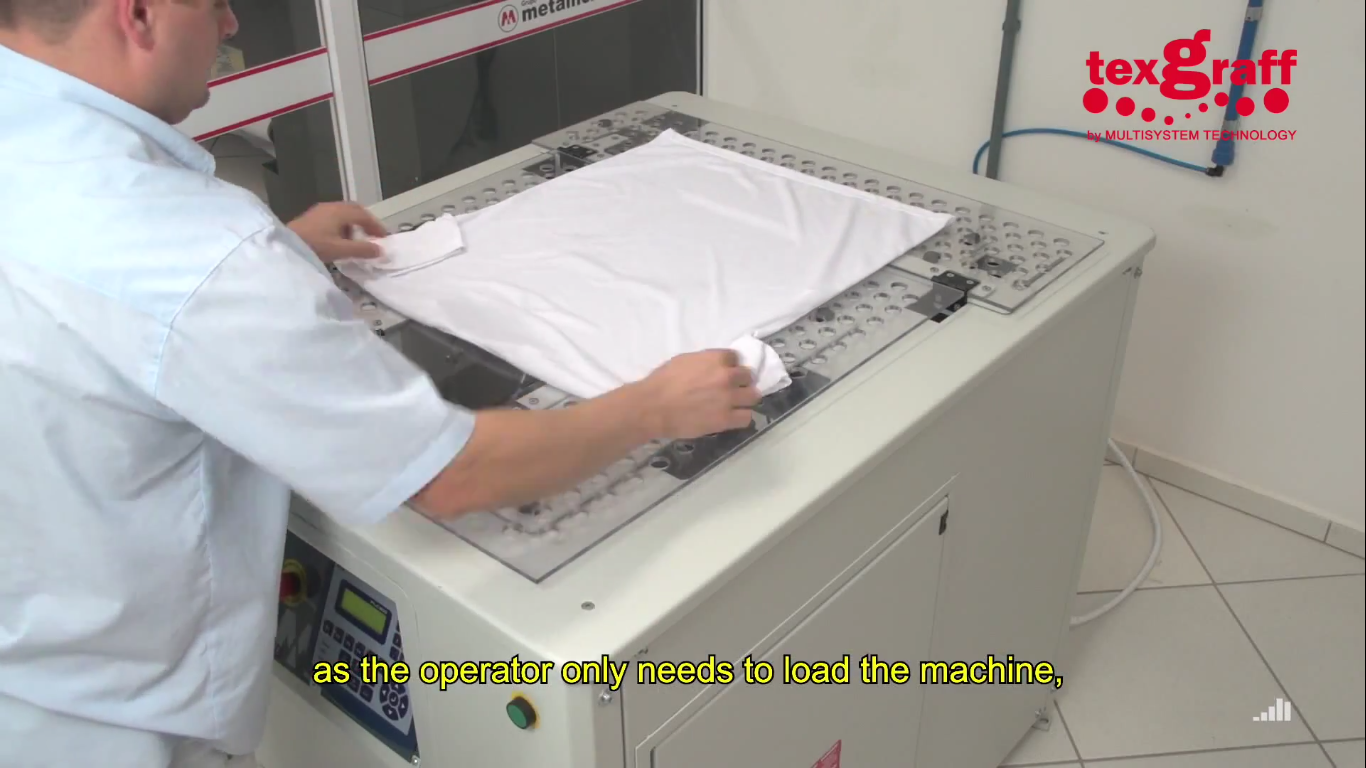
\includegraphics[width=\textwidth]
    		{figures/Intro_industrial_folding.png}
		    \caption{Automatic folding}        
		\end{subfigure} 
		\caption[Current clothes folding solutions available for garment folding]{Current clothes folding solutions available for garment folding. On the left, human workers folding clothes in a textile factory\footnotemark. On the right, an automated solution available in the market, manufactured by Texgraff\textcopyright.}
		\label{fig:current_solutions}
\end{figure}



Working with non-rigid objects such as clothes is a difficult task for robots, due to the complexity of modeling and manipulating deformable, thin objects. Clothes can be easily entangled when doing laundry, and recognizing individual garments and their category just from color or depth image analysis becomes an almost impossible task, due to occlusions amongst the cluttered clothes. Another challenging aspect when working with deformable objects is how to bring the object into a known configuration from an arbitrary initial state.

\footnotetext{Source:\stdurl{http://www.japantimes.co.jp/news/2012/12/19/reference/firms-move-some-eggs-out-of-china-basket/}, last accessed: \today.}

Extensive work can be found in literature about automated clothes folding once the garment category has been identified (that will be covered in the next chapter), as well as for modeling the garment for fold/wrinkle removal or selecting the most suitable grasping point/strategy. For that reason, this thesis focuses on how to unfold a clothing article that has been picked up from a pile of clothes and is placed on a flat surface. From that point, any of the existing approaches can be applied to fold the garment.

It is assumed that a clothing article has already been separated from the rest of the clothes to be folded, and placed on a flat surface. The garment could have been placed on that surface either by a robot or by a human coworker, allowing a collaborative folding pipeline in which a human and a robot can perform different parts of the folding process.
As our algorithm is not based on a geometrical model of the garment to be unfolded, it is general enough to be used with any category of garment, from towels and blankets to trousers or shirts, and with any number of folds. 
%
The presented approach consists in using a depth image from a single point of view to find regions of the garment overlapping other regions, which are considered to be folds. Then, all the possible candidate paths are studied to determine the unfolding direction. This is an iterative process to be repeated until the garment is fully unfolded.

\section{Objectives}
\label{intro_objectives}
The main objective pursued in this work is to develop an algorithm that can estimate the grasping and release points for a deformable object so that a manipulator robot can iteratively unfold a garment. Once unfolded, its garment category  and the folding sequence to apply can both be determined. From the aforehead mentioned \comment{algorithm} we can deduce the following specific objectives:

\begin{itemize}
	\item It should rely as little as possible in color or patterns present in the garment. This way, the algorithm is more robust and independent from the illumination conditions.
	\item It should provide a general method of detecting folds in deformable objects without a prior model of the garment to be unfolded. The absence of a prior model allows the algorithm to work with any kind of textile article, much as humans work with deformable objects.
	\item It should be able to estimate the best position of the grasping point, direction of movement, and release point in order to unfold the detected fold. An incorrect pick and place sequence would cause the garment to be more entangled that in the initial state, making the unfolding task even more complicated.
\end{itemize}


This work will aim to accomplish these specific objectives in order to solve the main objective. \comment{Stuuuuff}.

\section{Document Structure}
\label{intro_structure}

This section presents an overview of the concepts and contents contained in each of the chapters of this thesis. This way, the reader may consume this work in a linear fashion, from start to end, or concentrate on specific parts that are relevant to him. For that purpose the author has tried, whenever possible, to write chapters as much self-contained as possible.

\begin{itemize}
\item \textbf{Chapter \ref{state_of_the_art}} provides an overview of the current state of the different methods and techniques to achieve automatic robot garment folding. It includes techniques based both on modeling and manipulation, as well as works performed as part of the CloPeMa FP7 european project. This is chapter is recommended to obtain a general knowledge of other existing approaches that address the same problem as this work.
\item \textbf{Chapter \ref{architecture}} is related to the actual algorithm developed in this work. This chapter provides a general knowledge of the algorithm and its several stages, and therefore it is recommended that the reader reviews it to understand each concrete part in later chapters.
\item \textbf{Chapter \ref{garment_segmentation}} deals with the different steps that constitute the Garment Segmentation stage. This stage is required to determine which pixels of the input images correspond to the garment and which ones correspond to the background.
\item \textbf{Chapter \ref{garment_clustering}} describes the different steps involved in the Garment Depth Map clustering stage. In this stage the pixels from the input depth image are grouped in regions of similar depth, to determine overlapping parts of the garment.
\item \textbf{Chapter \ref{pick_and_place}} presents the different steps involved in the Garment Pick and Place Points stage, explaining how the different steps in this stage generate pick and place points for the humanoid robot to manipulate the garment.
\item \textbf{Chapter \ref{experiments_and_results}} is related to the different experiments performed to validate the algorithm. This chapter describes the experimental setup as well as the various experiments and results obtained from them.
\item \textbf{Chapter \ref{conclusions_and_future_work}} finally offers an analysis of the work and main contributions. The issues arised during the execution of this work are also mentioned, along with some lines of future work in order to address them.
\end{itemize}
